\documentclass[11pt,a4paper]{article}
\usepackage[utf8]{inputenc}
\usepackage[T1]{fontenc}
\usepackage{mathpazo}
\usepackage{amsmath,amssymb,amsthm,mathtools}
\usepackage[margin=1in]{geometry}
\usepackage{graphicx,booktabs,tabularx,hyperref,xcolor,fancyhdr,microtype}

\definecolor{primary}{RGB}{18, 53, 91}
\definecolor{accent}{RGB}{185, 28, 28}
\definecolor{slate}{RGB}{90, 101, 119}

\hypersetup{
  colorlinks=true,
  linkcolor=primary,
  citecolor=primary,
  urlcolor=primary,
  pdftitle={Classificacao EA com Vertices Isolados, Decomposicao Primaria K(G,Q) e Reducao por 1-Cociclo na Familia Quártica V2},
  pdfauthor={Auditoria Matematica Independente -- Projeto V2}
}

\setlength{\parskip}{6pt plus 2pt minus 1pt}
\setlength{\headheight}{14pt}

\pagestyle{fancy}
\fancyhf{}
\fancyhead[L]{\small\color{slate}\textit{Auditoria Matemática Independente e Novos Teoremas — Família Quártica V2}}
\fancyhead[R]{\small\color{slate}\textit{Outubro de 2026}}
\fancyfoot[C]{\small\color{slate}\thepage}
\renewcommand{\headrulewidth}{0.4pt}

\newtheorem{theorem}{Teorema}[section]
\newtheorem{proposition}[theorem]{Proposição}
\newtheorem{lemma}[theorem]{Lema}
\newtheorem{corollary}[theorem]{Corolário}
\theoremstyle{definition}
\newtheorem{definition}[theorem]{Definição}
\newtheorem{example}[theorem]{Exemplo}
\theoremstyle{remark}
\newtheorem{remark}[theorem]{Observação}

\newcommand{\takeaway}[2]{%
  \vspace{6pt}%
  \noindent\colorbox{primary!7}{%
    \parbox{\dimexpr\textwidth-2\fboxsep\relax}{%
      \vspace{4pt}\textbf{\color{primary}#1:}\hspace{0.5em}#2\vspace{4pt}%
    }%
  }%
  \vspace{6pt}%
}

\newcommand{\F}{\mathbb{F}_2}
\newcommand{\FF}{\mathbb{F}_{16}}
\newcommand{\Aut}{\operatorname{Aut}}
\newcommand{\Fix}{\operatorname{Fix}}
\newcommand{\Rad}{\operatorname{Rad}}
\newcommand{\Stab}{\operatorname{Stab}}
\newcommand{\Ind}{\operatorname{Ind}}
\newcommand{\Orb}{\operatorname{Orb}}
\newcommand{\Cen}{\operatorname{Cen}}
\newcommand{\Hom}{\operatorname{Hom}}
\newcommand{\GL}{\operatorname{GL}}
\newcommand{\GammaL}{\Gamma\mathrm{L}}
\newcommand{\Id}{\operatorname{Id}}

\title{\vspace{-1.2em}\textbf{\color{primary}Classificação Exata de Equivalências EA na Presença de Vértices Isolados, Decomposição Primária via Grafo de Dependências $K(G,Q)$ e Redução Algébrica por 1-Cociclo na Família Quártica V2}}
\author{\textbf{Auditoria Matemática Independente — Projeto V2}\\
\small Referência congelada: \texttt{contatofilipevono-rgb/hrsbf-bent-verification} (Outubro de 2026)}
\date{14 de outubro de 2026}

\begin{document}
\sloppy
\maketitle

\begin{abstract}
\noindent
Estudamos a família vetorial booleana quártica acoplada por dígrafos $(F_G)_i(x) = f(x_i) + x_{i,0}x_{i,1}\sum_{j:(i,j)\in E(G)} x_{j,0}$ sobre $V = (\F^8)^r$, onde $f = \Orb_8(01) + \Orb_8(0123) + \Orb_8(0125) + \Orb_8(0135) : \F^8 \to \F$ é a semente bent simétrica por rotação da construção V2 e $Q : (\F^8)^r \to \F^r$ é uma perturbação quadrática arbitrária ($\deg Q \le 2$). Além de auditar adversarialmente os resultados prévios, demonstramos cinco contribuições matemáticas originais:
(1) uma prova elementar e autocontida de recuperação intrínseca de blocos pelo radical de contração $\Rad_\Phi(u) = \{v \in V : i_{u\wedge v}\Phi = 0\}$, acompanhada da prova exata de $R_2(F_G+Q) = r$ e de uma fórmula fechada para o número $|\mathcal{M}_2(F_G+Q)|$ de subespaços $R_2$-maximais, que independe de $Q$ e distingue a orientação dos arcos ($G$ vs.\ $G^{\mathrm{op}}$);
(2) a decomposição estrutural exata $\Aut(\phi) = \mathcal{K}_Y^0 \rtimes (\langle C_3\rangle \times \langle P_5\rangle \rtimes \langle\sigma\rangle) \cong \F^4 \rtimes (C_{15} \rtimes C_8)$ de ordem $1920$ via geometria semilinear $\GammaL(2,4) \to \GammaL(1,16)$, reduzindo a prova de $\mathcal{G}_{\le 2}(f) = \langle P_5,\sigma\rangle \cong C_5 \rtimes C_8$ (ordem $40$) a apenas \textbf{duas testemunhas explícitas} ($C_3$ e $U_0 \in \mathcal{K}_Y^0$) por meio do 1-cociclo cúbico $\delta_3$, decomposição $P_5$-isotípica e Lema de Schur;
(3) o \textbf{Teorema de Classificação EA na Presença de Vértices Isolados}, que caracteriza necessária e suficentemente todas as equivalências EA quando $G$ possui $k = |I(G)| \ge 0$ vértices isolados, determina o grupo de gauge em produto corona $\mathcal{E}(G) \cong \Aut(G_{\mathrm{act}}) \times ((C_5 \rtimes C_8) \wr S_k)$ de ordem $|\Aut(G_{\mathrm{act}})|\,k!\,40^k$ e estabelece uma fórmula analítica fechada de Pólya--Burnside por Reciprocidade de Frobenius e monodromia de ciclos;
(4) o \textbf{Teorema de Decomposição Primária de Krull--Schmidt EA via $K(G,Q)$}, com algoritmo canônico em tempo $O(r^3)$, condensação triangular via $\vec{K}(G,Q)$ e fórmula de inversão de Möbius para o número exato de perturbações e classes EA indecomponíveis sobre dígrafos desconexos; e
(5) a separação rigorosa de escalas assintóticas em $\mathcal{N}_r$, provando a identidade polinomial $D - c_2(\tau) = 96r^2 - 204r + 144$ para transposições e a fórmula fechada de inclusão-exclusão em ciclos para dígrafos sem vértices isolados $I_r(\pi)$.
\end{abstract}

\takeaway{Síntese de Rigor e Proveniência}{Todas as demonstrações algébricas globais neste manuscrito estão integralmente provadas a partir das definições e reduzem os invariantes locais em $\F^8$ a certificados finitos verificados por três programas Python independentes (\texttt{CERTIFICADOS\_V2/}), sem depender de hipóteses não provadas ou de formalização Lean 4 incompleta.}

\vspace{8pt}
\section{Recuperação Elementar de Blocos e o Invariante de Flats $R_2$-Maximais}

Seja $V_0 = \F^8$ com base canônica $e_0,\dots,e_7$ e dual $e_0^*,\dots,e_7^*$. A semente escalar da construção V2 é a função booleana simétrica por rotação de grau $4$:
\begin{equation}\label{eq:seed}
  f(x) = \Orb_8(01) + \Orb_8(0123) + \Orb_8(0125) + \Orb_8(0135),
\end{equation}
que possui $8$ monômios quadráticos e $24$ monômios quárticos, peso de Hamming $\operatorname{wt}(f) = 120$ e espectro de Walsh-Hadamard constante $|W_f(\omega)| = 16$ (estritamente \emph{bent}). Sua quarta derivada direcional $\phi := D^4 f \in \Lambda^4(V_0^*)$ induz o operador simétrico de contração $C_\phi : \Lambda^2(V_0) \to \Lambda^2(V_0^*)$, $\langle C_\phi(u\wedge v), w_1\wedge w_2\rangle = \phi(u,v,w_1,w_2)$, de posto $22$ e nulidade $6$ em dimensão $\binom{8}{2} = 28$. Os $63$ bivetores não nulos de $\ker C_\phi$ distribuem-se em $3$ elementos de posto $4$ e $60$ elementos de posto $8$; em particular, $\ker C_\phi$ não contém bivetores simples de posto $2$ (\emph{propriedade Grassmann-free}):
\begin{equation}\label{eq:gf}
  \forall u,v \in V_0,\qquad i_{u\wedge v}\phi = 0 \iff u\wedge v = 0 \iff \dim_{\F}\operatorname{Span}\{u,v\} \le 1.
\end{equation}

Para $r \ge 1$, seja $V = \bigoplus_{i=1}^r V_i$ com $V_i \cong \F^8$, $W = \F^r$ com base $e_1,\dots,e_r$, e $G = ([r], E)$ um dígrafo sem laços ($E \subseteq \{ (i,j) \in [r]^2 : i \neq j \}$). A família V2 perturbada por $Q : V \to W$ ($\deg Q \le 2$) é dada coordenada a coordenada por
\begin{equation}\label{eq:family}
  (F_G + Q)_i(x) = f(x_i) + x_{i,0} x_{i,1} \sum_{j : (i,j) \in E} x_{j,0} + Q_i(x), \qquad i \in [r].
\end{equation}

Nos textos prévios, a recuperação dos blocos $V_1,\dots,V_r$ a partir de $\Phi := D^4(F_G+Q) = \sum_{i=1}^r e_i \otimes \phi_i$ invocava resultados gerais sobre idempotentes primitivos de álgebras de centroides. Apresentamos a seguir uma prova elementar e autocontida de 6 linhas baseada exclusivamente na propriedade Grassmann-free \eqref{eq:gf}, seguida da caracterização exata de todos os subespaços que realizam o índice relaxado de segunda derivada $R_2(F_G+Q) = r$.

\begin{theorem}[Recuperação Elementar de Blocos e Contagem Exata de Subespaços $R_2$-Maximais]\label{thm:block_and_R2}
Sejam $r \ge 1$, $G = ([r], E)$ um dígrafo sem laços qualquer (com ou sem vértices isolados) e $Q : V \to W$ com $\deg Q \le 2$.
\begin{enumerate}
  \item \textbf{Recuperação Intrínseca pelo Radical de Contração:} Para cada $u = (u_1,\dots,u_r) \in V$, defina o radical de segunda ordem da quarta derivada $\Phi = D^4(F_G+Q)$ por
  \[
    \Rad_\Phi(u) := \big\{ v \in V : i_{u\wedge v}\Phi = 0 \big\} = \big\{ v \in V : \forall w_1,w_2 \in V,\; \Phi(u,v,w_1,w_2) = 0 \big\}.
  \]
  Então $\Rad_\Phi(u) = \bigoplus_{i : u_i \neq 0} \F u_i$, de modo que $\dim_{\F} \Rad_\Phi(u) = |\{i \in [r] : u_i \neq 0\}|$. Consequentemente, a união dos blocos $\bigcup_{i=1}^r V_i = \{u \in V : \dim_{\F}\Rad_\Phi(u) \le 1\}$ e os blocos individuais $V_1,\dots,V_r$ (como subespaços lineares maximais contidos nessa união) são invariantes intrínsecos de $\Phi$. Toda equivalência linear $(B, A) \in \GL(W) \times \GL(V)$ que preserva $\Phi$ satisfaz $A(V_i) = V_{\pi(i)}$ e $B(e_{\pi(i)}) = e_i$ para uma única permutação $\pi \in S_r$.
  \item \textbf{Exatidão Universal de $R_2$:} O índice relaxado de segunda derivada $R_2(F) := \max\{\dim U : U \le V,\; \forall a,b \in U,\; D_a D_b F \text{ é constante}\}$ satisfaz exatamente
  \[
    R_2(F_G + Q) = r.
  \]
  \item \textbf{Caracterização e Fórmula Fechada de $\mathcal{M}_2(F_G+Q)$:} Um subespaço $U \le V$ de dimensão $r$ satisfaz $D_a D_b(F_G+Q) = \mathrm{const}$ para todos $a,b \in U$ se, e somente se, $U = \bigoplus_{i=1}^r \F v_i$ com $v_i \in V_i \setminus \{0\}$ tais que, para todo arco $(i,j) \in E(G)$, vale $(v_{i,0} = v_{i,1} = 0)$ ou $(v_{j,0} = 0)$. Em particular, o conjunto $\mathcal{M}_2(F_G+Q)$ de subespaços $R_2$-maximais é \textbf{independente de $Q$} e sua cardinalidade exata é um invariante EA de segunda ordem dado por
  \begin{equation}\label{eq:M2_count}
    |\mathcal{M}_2(F_G + Q)| = \sum_{A \subseteq [r]} 63^{r - |A|} \cdot 64^{|\{j \in A : N_G^-(j) \cap A \neq \emptyset\}|} \cdot 192^{|\{j \in A : N_G^-(j) \cap A = \emptyset\}|},
  \end{equation}
  onde $N_G^-(j) = \{i \in [r] : (i,j) \in E(G)\}$ é a vizinhança de entrada de $j$.
\end{enumerate}
\end{theorem}

\begin{proof}
(1) Como $e_1,\dots,e_r$ são linearmente independentes em $W$ e $i_{u\wedge v}\Phi = \sum_{i=1}^r e_i \otimes i_{u_i \wedge v_i}\phi_i$, temos $i_{u\wedge v}\Phi = 0$ se e somente se $i_{u_i \wedge v_i}\phi_i = 0$ para todo $i \in [r]$. Pela propriedade Grassmann-free \eqref{eq:gf}, isso equivale a $u_i \wedge v_i = 0$ para todo $i \in [r]$, isto é, $v_i \in \F u_i$ para cada $i$. Logo $\Rad_\Phi(u) = \bigoplus_{i : u_i \neq 0} \F u_i$, cuja dimensão é exatamente o número de blocos nos quais $u$ tem projeção não nula. Dois vetores não nulos $u, u'$ com $\dim\Rad_\Phi(u) = \dim\Rad_\Phi(u') = 1$ pertencem ao mesmo bloco $V_i$ se e somente se $\dim\Rad_\Phi(u+u') \le 1$. Isso recupera $\{V_1,\dots,V_r\}$ sem ambiguidade, e $\operatorname{Im}(\Phi|_{V_i^4}) = \F e_i$ força $B(e_{\pi(i)}) = e_i$.

(2) Seja $U \le V$ tal que $D_a D_b(F_G+Q)$ é constante para todos $a,b \in U$. Derivando mais duas vezes nas direções $c,d \in V$, obtemos $\Phi(a,b,c,d) = D_c D_d D_a D_b(F_G+Q) = 0$, ou seja, $i_{a\wedge b}\Phi = 0$. Pelo item (1), $a_i \wedge b_i = 0$ para todo $i \in [r]$ e todos $a,b \in U$. Portanto, a projeção $\pi_i(U) \le V_i$ tem dimensão $\dim_{\F}\pi_i(U) \le 1$ para cada $i \in [r]$. Como $U \le \bigoplus_{i=1}^r \pi_i(U)$, segue-se que $\dim U \le \sum_{i=1}^r \dim\pi_i(U) \le r$. Reciprocamente, tomando $v_i = e_{i,2} \in V_i$ (onde $v_{i,0} = v_{i,1} = 0$) e $U = \bigoplus_{i=1}^r \F e_{i,2}$, temos $\dim U = r$; para quaisquer $a,b \in U$, $a_i$ e $b_i$ são colineares sobre $\F$ ($a_i = 0$, $b_i = 0$ ou $a_i = b_i$), logo $D_{a_i}D_{b_i}f(x_i) \equiv 0$, os termos cúbicos anulam-se pois $a_{i,0}=a_{i,1}=b_{i,0}=b_{i,1}=0$, e $D_a D_b Q$ é constante por ser $\deg Q \le 2$. Logo $R_2(F_G+Q) = r$.

(3) Se $\dim U = r$ e $\dim\pi_i(U) \le 1$ para todo $i$, a inclusão $U \le \bigoplus_{i=1}^r \pi_i(U)$ força a igualdade $U = \bigoplus_{i=1}^r \F v_i$ com $v_i \in V_i \setminus \{0\}$ únicos. Pela bilinearidade de $(a,b) \mapsto D_a D_b(F_G+Q)$ modulo constantes e pelo fato de $D_{v_i}D_{v_i}(F_G+Q) \equiv 0$, $U \in \mathcal{M}_2(F_G+Q)$ se e somente se $D_{v_i}D_{v_j}(F_G+Q)$ é constante para todo par $i \neq j$. Como $D_{v_i}D_{v_j}f(x_m) \equiv 0$ (já que $f(x_m)$ depende apenas de um bloco) e $D_{v_i}D_{v_j}Q = \mathrm{const}$, resta apenas o acoplamento cúbico $C_m(x) = x_{m,0}x_{m,1}\sum_{(m,k)\in E} x_{k,0}$. Na coordenada $m=i$, o único termo que envolve simultaneamente $V_i$ e $V_j$ ocorre quando $(i,j) \in E$, contribuindo com
\[
  D_{v_i}D_{v_j}(x_{i,0}x_{i,1}x_{j,0}) = \big(v_{i,0}x_{i,1} + v_{i,1}x_{i,0} + v_{i,0}v_{i,1}\big) v_{j,0}.
\]
Essa função afim de $x_i$ é constante se, e somente se, sua parte linear $(v_{i,0}x_{i,1} + v_{i,1}x_{i,0})v_{j,0}$ é identicamente nula, isto é, $(v_{i,0},v_{i,1}) = (0,0)$ ou $v_{j,0} = 0$. Particionando $V_i \setminus \{0\}$ ($255$ vetores) em $S_0 = \{v \neq 0 : v_0 = v_1 = 0\}$ ($2^6 - 1 = 63$ vetores) e $S_0^c = \{v : (v_0,v_1) \neq (0,0)\}$ ($192$ vetores, dos quais $64$ satisfazem $v_0=0, v_1=1$ e $128$ satisfazem $v_0=1$), e condicionando sobre o subconjunto $A = \{i \in [r] : v_i \in S_0^c\}$, todo $j \notin A$ já cumpre $v_{j,0}=0$, enquanto um vértice $j \in A$ fica restrito aos $64$ vetores com $v_{j,0}=0$ se e somente se possui algum vizinho de entrada $i \in A$ ($(i,j) \in E$), tendo $192$ escolhas caso contrário. Isso demonstra \eqref{eq:M2_count}.
\end{proof}

\begin{remark}[Assimetria Direcional de Segunda Ordem]
A fórmula \eqref{eq:M2_count} revela que $|\mathcal{M}_2(F_G+Q)|$ distingue dígrafos transpostos $G$ e $G^{\mathrm{op}}$ que possuem o mesmo grafo subjacente e o mesmo grupo de automorfismos: para $r=3$, a estrela divergente $G_{\mathrm{out}} = \{0\to 1, 0\to 2\}$ tem $|\mathcal{M}_2| = 7.193.343$, enquanto a estrela convergente $G_{\mathrm{in}} = \{1\to 0, 2\to 0\}$ tem $|\mathcal{M}_2| = 8.766.207$.
\end{remark}

\vspace{8pt}
\section{Estrutura Algébrica de $\Aut(\phi)$ e Redução por 1-Cociclo e Lema de Schur (C3)}

Os três bivetores de posto $4$ em $\ker C_\phi$ possuem todos o mesmo suporte intrínseco de dimensão $4$, $U = \Fix(\sigma^4) = \operatorname{Span}\{u_i := e_i + e_{i+4} : 0 \le i \le 3\}$, onde $\sigma(e_i) = e_{i+1 \pmod 8}$. Completando a base de $V_0 = U \oplus E$ com $E = \operatorname{Span}\{e_0,e_1,e_2,e_3\}$, qualquer $A \in \Aut(\phi)$ preserva $U$ e escreve-se na forma triangular em blocos
\begin{equation}\label{eq:block_form}
  A = \begin{pmatrix} P & Y \\ 0 & Q \end{pmatrix}, \qquad P \in \GL(U),\; Q \in \GL(E),\; Y \in \Hom(E, U) \cong \F^{4\times 4}.
\end{equation}

\begin{theorem}[Decomposição Semilinear $\GammaL(1,16)$ e Prova de Duas Testemunhas via Lema de Schur]\label{thm:c3_structure}
Na decomposição intrínseca $V_0 = U \oplus E$:
\begin{enumerate}
  \item \textbf{Anulação de Bidegraus e Igualdade Diagonal $P = Q$:} A forma $\phi = D^4 f$ possui componentes de bidegrau $(4,0)$ e $(3,1)$ identicamente nulas em $U \oplus E$. O componente $(2,2)$, $M : \Lambda^2(U) \times \Lambda^2(E) \to \F$, tem posto $4$ e núcleos esquerdo e direito iguais a $K_L = K_R = \operatorname{Span}\{\omega_1, \omega_2\}$ de dimensão $2$, onde $\omega_1 = e_{02}+e_{03}+e_{12}$ e $\omega_2 = e_{01}+e_{13}+e_{23}$ definem um \emph{spread} desarguesiano $\mathbb{F}_4^2$ cujo estabilizador em $\GL(4,2)$ é $\GammaL(2,4)$ de ordem $360$. O componente $(1,3)$, $N : U \times \Lambda^3(E) \to \F$, força \textbf{exatamente $P = Q$} e reduz a projeção diagonal $\{P : (P,P,Y) \in \Aut(\phi)\}$ ao grupo semilinear unidimensional $\GammaL(1,16) = \FF^\times \rtimes \operatorname{Gal}(\FF/\F) \cong C_{15} \rtimes C_4$ de ordem $60$.
  \item \textbf{Decomposição em Produto Semidireto de $\Aut(\phi)$:} O núcleo da projeção $\pi : \Aut(\phi) \to \GammaL(1,16)$ é o subgrupo abeliano elementar de cisalhamentos $\mathcal{K}_Y = \{I_8 + Y : Y \in \mathcal{K}_Y\} \cong \F^5$ de ordem $32$, que consiste exatamente na identidade e nas $31$ únicas involuções de $\Aut(\phi)$. Sob conjugação pelo elemento $P_5$ de ordem $5$, $\mathcal{K}_Y$ decompõe-se em $\mathcal{K}_Y = Z(\Aut(\phi)) \oplus \mathcal{K}_Y^0$, onde $Z(\Aut(\phi)) = \langle\sigma^4\rangle \cong C_2$ é o centro de $\Aut(\phi)$ e $\mathcal{K}_Y^0 := [\mathcal{K}_Y, P_5] \cong \F^4$ (ordem $16$) é um $\F[P_5]$-módulo irredutível normal em $\Aut(\phi)$. Como $\sigma^4 \in \langle\sigma\rangle \cong C_8$, obtém-se a decomposição global exata em produto semidireto:
  \begin{equation}\label{eq:aut_semidirect}
    \Aut(\phi) = \mathcal{K}_Y^0 \rtimes (\langle C_3 \rangle \times \langle P_5 \rangle \rtimes \langle \sigma \rangle) \cong \F^4 \rtimes (C_{15} \rtimes C_8), \quad |\Aut(\phi)| = 1920,
  \end{equation}
  com relações $\sigma C_3 \sigma^{-1} = C_3^2$, $\sigma P_5 \sigma^{-1} = P_5^3$, $C_3 P_5 = P_5 C_3$ e $[C_3, \mathcal{K}_Y^0] = 1$.
  \item \textbf{Redução por 1-Cociclo e Duas Testemunhas para $\mathcal{G}_{\le 2}(f)$:} A aplicação de translação cúbica $\iota_\phi : V_0 \to \Lambda^3(V_0^*)$, $a \mapsto [f(x+a)+f(x)]_3 = i_a\phi$, é linear e injetora ($\dim\operatorname{Im}(\iota_\phi) = 8$). A aplicação $\delta_3 : \Aut(\phi) \to \Lambda^3(V_0^*)$, $\delta_3(A) := [f(Ax)+f(x)]_3 = [f_4(Ax)+f_4(x)]_3$, satisfaz a identidade exata de 1-cociclo
  \begin{equation}\label{eq:cocycle}
    \delta_3(AB) = B^*\delta_3(A) + \delta_3(B) \qquad \forall A,B \in \Aut(\phi),
  \end{equation}
  e um par $(A,a) \in \Aut(\phi) \times V_0$ satisfaz $\deg(f(Ax+a)+f(x)) \le 2$ se e somente se $\delta_3(A) = i_a\phi \in \operatorname{Im}(\iota_\phi)$. Como $\delta_3(P_5) = \delta_3(\sigma) = 0$, o subgrupo $G_{40} := \langle P_5, \sigma \rangle \cong C_5 \rtimes C_8$ de ordem $40$ preserva $f$ identicamente. Sobre o complemento normal abeliano $N_{48} := \mathcal{K}_Y^0 \times \langle C_3 \rangle \cong \F^4 \times C_3$, a igualdade $\mathcal{G}_{\le 2}(f) = G_{40}$ (e $a = 0$) decorre \textbf{sem enumeração exaustiva} de apenas duas verificações pontuais:
  \begin{enumerate}
    \item[(a)] $\delta_3(C_3) \neq 0$ (testemunha: o monômio $x_0 x_1 x_3$ tem coeficiente $1$ em $\delta_3(C_3)$), o que elimina $C_3$ e $C_3^2$ porque $C_3$ comuta com $P_5$, logo $\delta_3(C_3) \in \Fix_{\Lambda^3(V_0^*)}(P_5)$, enquanto $\operatorname{Im}(\iota_\phi) \cong V_0$ e $\delta_3(\mathcal{K}_Y^0)$ residem inteiramente na componente $\Phi_5$-isotípica (pois $\Fix_{V_0}(P_5) = \{0\}$);
    \item[(b)] $\delta_3(U_0) \notin \operatorname{Im}(\iota_\phi)$ para um único elemento não trivial $U_0 \in \mathcal{K}_Y^0 \setminus \{I_8\}$ (testemunha: monômio $x_0 x_1 x_2$), o que pelo \textbf{Lema de Schur} implica a injetividade do homomorfismo $\F[P_5]$-linear induzido $\bar{\delta}_3 : \mathcal{K}_Y^0 \to \Lambda^3(V_0^*)/\operatorname{Im}(\iota_\phi)$ sobre o módulo simples $\mathcal{K}_Y^0 \cong \F^4$.
  \end{enumerate}
\end{enumerate}
\end{theorem}

\begin{proof}
A verificação algébrica das matrizes $M$ ($6\times 6$) e $N$ ($4\times 4$) mostra que para $(P,Q) = (I_4, I_4)$, o sistema linear $(1,3)$ em $Y \in \F^{4\times 4}$ tem posto $10$ e núcleo $W_0$ de dimensão $6$, sobre o qual a condição $(0,4)$ reduz-se a uma única funcional linear não nula, definindo o hiperplano $\mathcal{K}_Y \le W_0$ de dimensão $5$ ($32$ matrizes). Como qualquer $(P,Q,Y) \in \Aut(\phi)$ multiplica $\mathcal{K}_Y$ à esquerda mantendo $(P,Q)$ fixo, $|\Aut(\phi)| = 32 \times |\operatorname{Im}(\pi)| = 32 \times 60 = 1920$.

Para a redução do item (3), note que para $x \mapsto x+a$, a expansão de Taylor sobre $\F$ de um polinômio de grau $4$ fornece $[f(x+a)+f(x)]_3 = i_a(D^4 f) = i_a\phi$, que é linear em $a$; se $i_a\phi = 0$ para $a \neq 0$, então $i_{a\wedge b}\phi = 0$ para todo $b$, contradizendo \eqref{eq:gf}. Para $A,B \in \Aut(\phi)$, $f(ABx)+f(x) = B^*(f(Ay)+f(y)) + (f(Bx)+f(x))$, e como $A \in \Aut(\phi)$ anula a parte homogênea de grau $4$ de $f(Ay)+f(y)$, o operador linear $B^*$ comuta com a extração da parte homogênea de grau $3$, provando \eqref{eq:cocycle}. Pela decomposição $\Aut(\phi) = N_{48} \rtimes G_{40}$ e $\delta_3|_{G_{40}} = 0$, temos $\delta_3(n g) = g^*\delta_3(n)$ para $n \in N_{48}, g \in G_{40}$. Como $\operatorname{Im}(\iota_\phi)$ é $\Aut(\phi)$-invariante, $ng \in \mathcal{G}_{\le 2}(f) \iff \delta_3(n) \in \operatorname{Im}(\iota_\phi)$. Escrevendo $n = u C_3^j$ com $u \in \mathcal{K}_Y^0$ e $j \in \{0,1,2\}$, a relação $C_3 P_5 = P_5 C_3$ implica que $\delta_3(C_3^j) \in \Fix_{\Lambda^3(V_0^*)}(P_5)$. Por outro lado, o polinômio característico de $P_5$ em $V_0$ é $\Phi_5(t)^2 = (t^4+t^3+t^2+t+1)^2$, logo $\Fix_{V_0}(P_5) = \{0\}$ e $\operatorname{Im}(\iota_\phi) = \iota_\phi(V_0)$ está contido no núcleo de $1+P_5^*+(P_5^*)^2+(P_5^*)^3+(P_5^*)^4$ (componente $\Phi_5$-isotípica), que tem interseção nula com $\Fix_{\Lambda^3(V_0^*)}(P_5)$ pois $\gcd(t-1, \Phi_5(t)) = 1$ em $\F[t]$. Do mesmo modo, para $u,v \in \mathcal{K}_Y^0$, como $v = I_8 + Y_v$ atua trivialmente em $U$ e em $V_0/U$, $v^*$ atua trivialmente em $\delta_3(u)$, logo $\delta_3(uv) = \delta_3(u) + \delta_3(v)$, isto é, $\delta_3|_{\mathcal{K}_Y^0} : \mathcal{K}_Y^0 \to \Lambda^3(V_0^*)$ é estritamente $\F$-linear e $P_5$-equivariante. Assim, $\delta_3(u C_3^j) = (C_3^j)^*\delta_3(u) + \delta_3(C_3^j) \in \operatorname{Im}(\iota_\phi)$ força separadamente $\delta_3(C_3^j) = 0$ (excluindo $j=1,2$ pela Testemunha 1) e $\bar{\delta}_3(u) = 0$ em $\Lambda^3(V_0^*)/\operatorname{Im}(\iota_\phi)$. Como $\mathcal{K}_Y^0 \cong \F^4$ é um $\F[P_5]$-módulo simples ($\Phi_5(t)$ é irredutível sobre $\F$), o Lema de Schur garante que $\ker(\bar{\delta}_3|_{\mathcal{K}_Y^0})$ é $\{I_8\}$ ou $\mathcal{K}_Y^0$; a Testemunha 2 ($U_0 \in \mathcal{K}_Y^0$ com $\bar{\delta}_3(U_0) \neq 0$) força $\ker(\bar{\delta}_3|_{\mathcal{K}_Y^0}) = \{I_8\}$. Finalmente, as órbitas de $e_0^*$ e $e_0^*\wedge e_1^*$ sob $G_{40}$ têm ambas cardinalidade $40 = |G_{40}|$, logo seus estabilizadores são triviais pelo Teorema Órbita-Estabilizador.
\end{proof}

\vspace{8pt}
\section{Classificação EA Exata na Presença de Vértices Isolados e Fórmula de Burnside por Monodromia (C1)}

O teorema de ultra-rigidez da versão anterior exigia a hipótese restritiva de que $G$ e $H$ não possuíssem vértices isolados. Removemos agora essa restrição, determinando exatamente todos os graus de liberdade EA quando existem vértices isolados e derivando uma fórmula analítica fechada para a contagem de classes EA.

Para um dígrafo sem laços $G = ([r], E)$, denote por $I(G) := \{i \in [r] : \deg_G^+(i) = \deg_G^-(i) = 0\}$ o conjunto de seus \textbf{vértices isolados} ($k := |I(G)|$) e por $V_{\mathrm{act}}(G) := [r] \setminus I(G)$ o conjunto de seus \textbf{vértices ativos}, com subdígrafo induzido $G_{\mathrm{act}} := G[V_{\mathrm{act}}(G)]$. Fixamos a convenção matricial canônica: para $\pi \in S_r$, $P_\pi \in \GL(W)$ é definida por $P_\pi(e_i) = e_{\pi(i)}$ (logo $(P_\pi w)_{\pi(i)} = w_i$ e $(P_\pi^{-1} w)_i = w_{\pi(i)}$).

\begin{theorem}[Classificação EA Completa com Vértices Isolados e Grupo em Produto Corona]\label{thm:c1_isolated}
Sejam $r \ge 1$, $G = ([r], E)$ e $H = ([r], E')$ dígrafos sem laços arbitrários (com $k = |I(G)| \ge 0$ vértices isolados), e $Q, Q' : V \to W$ aplicações de grau algébrico $\le 2$.
\begin{enumerate}
  \item \textbf{Caracterização Necessária e Suficiente:} Uma quádrupla $(B, A, a_0, L + c_0)$ com $B \in \GL(W)$, $A \in \GL(V)$, $a_0 \in V$ e $\deg(L+c_0) \le 1$ realiza a equivalência EA
  \begin{equation}\label{eq:ea_rel}
    (F_H + Q')(x) = B\big((F_G + Q)(Ax + a_0)\big) + L(x) + c_0
  \end{equation}
  se, e somente se, valem simultaneamente:
  \begin{enumerate}
    \item[(i)] Existe um isomorfismo de dígrafos $\pi : H \to G$ (que necessariamente aplica $I(H)$ bijetivamente sobre $I(G)$ e $V_{\mathrm{act}}(H)$ sobre $V_{\mathrm{act}}(G)$) tal que $B = P_\pi^{-1}$;
    \item[(ii)] $a_0 = 0$ \textbf{globalmente} (inclusive em todos os blocos correspondentes a vértices isolados);
    \item[(iii)] $A = (P_\pi \otimes I_8)\,\operatorname{diag}(A_1, \dots, A_r)$, onde
    \[
      A_i = I_8 \quad \forall i \in V_{\mathrm{act}}(H), \qquad\text{e}\qquad A_i \in \mathcal{G}_{\le 2}(f) \cong C_5 \rtimes C_8 \quad \forall i \in I(H);
    \]
    \item[(iv)] As partes quadráticas homogêneas satisfazem a conjugação exata
    \begin{equation}\label{eq:quad_conj_iso}
      [Q']_2(x) = P_\pi^{-1} [Q]_2\big((P_\pi \otimes I_8)\operatorname{diag}(A_1,\dots,A_r) x\big),
    \end{equation}
    e $L(x) + c_0 = [Q']_{\le 1}(x) + P_\pi^{-1}[Q]_{\le 1}(Ax)$.
  \end{enumerate}
  \item \textbf{Grupo de Gauge EA em Produto Corona:} Para um dígrafo fixo $G$ com $k = |I(G)|$ vértices isolados, o grupo $\mathcal{E}(G)$ de pares lineares $(B, A)$ que preservam $F_G$ a menos de termos quadráticos (e que, de fato, preservam $F_G$ \textbf{exatamente}, $B F_G(Ax) = F_G(x)$) decompõe-se como o produto direto do grupo de automorfismos da parte ativa com o \textbf{produto corona} (\emph{wreath product}) de $C_5 \rtimes C_8$ por $S_k$:
  \begin{equation}\label{eq:wreath_group}
    \mathcal{E}(G) \;\cong\; \Aut(G_{\mathrm{act}}) \times \big(\mathcal{G}_{\le 2}(f) \wr S_k\big) \;\cong\; \Aut(G_{\mathrm{act}}) \times \big((C_5 \rtimes C_8) \wr S_k\big),
  \end{equation}
  de ordem exata $|\mathcal{E}(G)| = |\Aut(G_{\mathrm{act}})| \cdot k! \cdot 40^k$. Para cada $Q$, o grupo de automorfismos EA de $F_G+Q$ (módulo adições afins) é $\Aut_{\mathrm{EA}}(F_G+Q) = \Stab_{\mathcal{E}(G)}([Q]_2)$.
\end{enumerate}
\end{theorem}

\begin{proof}
Aplicando $D^4$ a \eqref{eq:ea_rel}, o Teorema~\ref{thm:block_and_R2}(1) garante a existência de uma única permutação $\pi \in S_r$ tal que $B = P_\pi^{-1}$ e $A = (P_\pi \otimes I_8)\operatorname{diag}(A_1,\dots,A_r)$ com $A_i \in \Aut(\phi)$. Escrevendo $a_0 = (P_\pi \otimes I_8)(b_1,\dots,b_r)$ com $b_i \in V_i$, a coordenada $i$ de $B(F_G+Q)(Ax+a_0)$ é $(F_G+Q)_{\pi(i)}(y)$ avaliada em $y_{\pi(j)} = A_j x_j + b_j$.

Tomando a terceira derivada direcional intra-bloco $D_{u}D_{v}D_{w}$ com $u,v,w \in V_i$ (para \textbf{qualquer} $i \in [r]$, isolado ou ativo), todos os acoplamentos cúbicos $y_{\pi(i),0}y_{\pi(i),1}y_{k,0}$ ($k \neq \pi(i)$) têm grau $\le 2$ nas variáveis do bloco $\pi(i)$ e portanto se anulam sob $D_u D_v D_w$, assim como $Q$ e $Q'$. Resta a identidade exata em $V_i$:
\[
  D_u D_v D_w\big(f(A_i x_i + b_i)\big) = D_u D_v D_w f(x_i) \quad \forall u,v,w \in V_i \implies \deg\big(f(A_i x_i + b_i) + f(x_i)\big) \le 2.
\]
Pelo Teorema~\ref{thm:c3_structure}(3), isso força $b_i = 0$ e $A_i \in \mathcal{G}_{\le 2}(f)$ para \textbf{todo} $i \in [r]$ (logo $a_0 = 0$ globalmente e $f(A_i x_i) = f(x_i)$ identicamente).

Em seguida, para cada par ordenado $(i,j)$ com $i \neq j$, a terceira derivada mista $D_{u_1}D_{u_2}D_w$ com $u_1,u_2 \in V_i$ e $w \in V_j$ na $i$-ésima coordenada de saída anula $f(x_i)$ e $Q, Q'$, isolando exatamente o tensor de posto $1$ do arco $(i,j)$:
\[
  \mathbf{1}_{(i,j) \in E(H)}\, (e_0^* \wedge e_1^*)(u_1, u_2)\, e_0^*(w) = \mathbf{1}_{(\pi(i),\pi(j)) \in E(G)}\, (A_i^*(e_0^* \wedge e_1^*))(u_1, u_2)\, (A_j^* e_0^*)(w).
\]
Como $(e_0^*\wedge e_1^*) \otimes e_0^* \neq 0$, concluímos que $(i,j) \in E(H) \iff (\pi(i),\pi(j)) \in E(G)$, ou seja, $\pi : H \to G$ é um isomorfismo de dígrafos. Além disso, para todo arco $(i,j) \in E(H)$, temos $A_i^*(e_0^*\wedge e_1^*) = e_0^*\wedge e_1^*$ e $A_j^*(e_0^*) = e_0^*$; como os estabilizadores em $\mathcal{G}_{\le 2}(f)$ são triviais (Teorema~\ref{thm:c3_structure}), segue-se que $A_i = I_8$ e $A_j = I_8$. Portanto, $A_i = I_8$ para todo vértice ativo $i \in V_{\mathrm{act}}(H)$.

Por outro lado, se $i \in I(H)$ é um vértice isolado, ele não figura como origem nem como destino de nenhum arco, logo as derivadas mistas não impõem qualquer restrição adicional a $A_i \in \mathcal{G}_{\le 2}(f)$. Como todo $A_i \in \mathcal{G}_{\le 2}(f)$ satisfaz a igualdade funcional exata $f(A_i x_i) = f(x_i)$ (sem produzir sequer resíduos de grau $\le 2$) e não há termos cúbicos incidentes em $i$, vale a identidade exata $P_\pi^{-1} F_G(Ax) = F_H(x)$ para qualquer escolha independente de $(A_i)_{i \in I(H)} \in \mathcal{G}_{\le 2}(f)^k$. Subtraindo $F_H(x) = P_\pi^{-1}F_G(Ax)$ de \eqref{eq:ea_rel}, resta $Q'(x) = P_\pi^{-1}Q(Ax) + L(x) + c_0$, que equivale a \eqref{eq:quad_conj_iso}.
\end{proof}

Para enumerar as classes EA de $F_G + Q$ quando $k = |I(G)| \ge 1$, precisamos calcular a dimensão fixa $c_2(g) := \dim_{\F}\Fix_{\mathcal{Q}_r}(g)$ no espaço quadrático $\mathcal{Q}_r = W \otimes \Lambda^2(V^*)$ de dimensão $D = r\binom{8r}{2} = 4r^2(8r-1)$ para elementos gerais $g = (\pi, (A_1,\dots,A_r)) \in \mathcal{E}(G)$, nos quais $A_i \in C_5 \rtimes C_8$ não são matrizes de permutação de coordenadas (por exemplo, quando $5 \mid \operatorname{ord}(A_i)$). O teorema a seguir resolve esse problema em forma fechada.

\begin{theorem}[Redução de Pólya--Burnside por Reciprocidade de Frobenius e Monodromia de Ciclos]\label{thm:c1_burnside}
Seja $g = (\pi, (A_1,\dots,A_r)) \in \mathcal{E}(G)$, e sejam $C_1,\dots,C_s$ os ciclos disjuntos de $\pi$ em $[r]$, de comprimentos $\ell_1,\dots,\ell_s$. Para cada ciclo $C_\alpha = (i_0, i_1=\pi(i_0), \dots, i_{\ell_\alpha-1})$, defina sua \textbf{monodromia de ciclo} $M_\alpha := A_{i_0} A_{i_{\ell_\alpha-1}} \cdots A_{i_1} \in \mathcal{G}_{\le 2}(f)$ e sua ordem $m_\alpha := \operatorname{ord}(M_\alpha) \in \{1, 2, 4, 5, 8, 10\}$ (sendo $m_\alpha = 1$ para todo ciclo contido em $V_{\mathrm{act}}(G)$).
\begin{enumerate}
  \item \textbf{Identidade de Reciprocidade de Frobenius:} Como $W = \bigoplus_{\alpha=1}^s W_{C_\alpha}$ com $W_{C_\alpha} \cong \Ind_{\langle g^{\ell_\alpha}\rangle}^{\langle g\rangle}(\F)$, vale o isomorfismo canônico $\Fix_{W_{C_\alpha} \otimes \Lambda^2(V^*)}(g) \cong \Fix_{\Lambda^2(V^*)}(g^{\ell_\alpha})$, de modo que
  \begin{equation}\label{eq:frob_c2}
    c_2(g) = \dim_{\F}\Fix_{\mathcal{Q}_r}(g) = \sum_{\alpha=1}^s \dim_{\F}\Fix_{\Lambda^2(V^*)}\!\big(g^{\ell_\alpha}\big),
  \end{equation}
  e $c_2(g)$ depende \textbf{exclusivamente} da lista de pares $(\ell_\beta, m_\beta)_{\beta=1}^s$.
  \item \textbf{Fórmulas Fechadas Exatas de Decomposição Jordan--Ciclotômica:} Sob a potência $T = g^L$ ($L = \ell_\alpha$), cada ciclo $(\ell_\beta, m_\beta)$ parte-se em $g_\beta = \gcd(\ell_\beta, L)$ ciclos de comprimento $\ell'_\beta = \ell_\beta / g_\beta$ e ordem de monodromia $m'_\beta = m_\beta / \gcd(m_\beta, L / g_\beta)$. Listando todos os ciclos refinados de $T = g^L$ como $(l_I, m_I)_{I=1}^t$, temos
  \begin{equation}\label{eq:lambda2_decomp}
    \dim_{\F}\Fix_{\Lambda^2(V^*)}(g^L) = \sum_{I=1}^t \phi_{\mathrm{intra}}(l_I, m_I) + \sum_{1 \le I < J \le t} \phi_{\mathrm{inter}}(l_I, m_I; l_J, m_J),
  \end{equation}
  onde as funções universais $\phi_{\mathrm{intra}}$ e $\phi_{\mathrm{inter}}$ são dadas analiticamente por:
  \begin{equation}\label{eq:phi_intra}
    \phi_{\mathrm{intra}}(l, m) = \begin{cases}
      32l & \text{se } m = 1 \text{ e } l \text{ é par},\\
      32l - 4 & \text{se } m = 1 \text{ e } l \text{ é ímpar},\\
      32l / m & \text{se } m \in \{2, 4, 8\},\\
      40l / m & \text{se } m \in \{5, 10\},
    \end{cases}
  \end{equation}
  e, decompondo cada par $(l, m)$ na quadrupla $(n, A, B, s)$ dada por $(8/m, (lm)_2, (lm)_{2'}, 1)$ se $m \in \{1,2,4,8\}$ e $(10/m, (lm/5)_2, l_{2'}, 5)$ se $m \in \{5,10\}$ (onde $x_2 = 2^{v_2(x)}$ e $x_{2'} = x/x_2$),
  \begin{equation}\label{eq:phi_inter}
    \phi_{\mathrm{inter}}(l_1, m_1; l_2, m_2) = n_1 n_2 \min(A_1, A_2)\, \Delta(B_1, s_1; B_2, s_2),
  \end{equation}
  onde $\Delta(B_1,1; B_2,1) = \gcd(B_1,B_2)$, $\Delta(B_1,5; B_2,1) = \gcd(5B_1,B_2) - \gcd(B_1,B_2)$, $\Delta(B_1,1; B_2,5) = \gcd(B_1,5B_2) - \gcd(B_1,B_2)$, e $\Delta(B_1,5; B_2,5) = \gcd(5B_1,5B_2) - \gcd(B_1,5B_2) - \gcd(5B_1,B_2) + \gcd(B_1,B_2)$.
  \item \textbf{Contagem Exata de Classes EA com Vértices Isolados:} Consequentemente, para qualquer dígrafo $G$ com $k = |I(G)|$ vértices isolados, a soma sobre as $40^k$ tuplas em $\mathcal{G}_{\le 2}(f)^k$ colapsa para as ordens de monodromia com pesos $w(1)=1, w(2)=1, w(4)=10, w(5)=4, w(8)=20, w(10)=4$:
  \begin{equation}\label{eq:burnside_iso}
    \textstyle N_{\mathrm{EA}}(G) = \frac{1}{|\Aut(G_{\mathrm{act}})|\,k!} \sum_{\pi_{\mathrm{act}} \in \Aut(G_{\mathrm{act}})} \sum_{\pi_{\mathrm{iso}} \in S_k} \sum_{\mathbf{m}} \Big(\prod_{\beta=1}^{c(\pi_{\mathrm{iso}})} \frac{w(m_\beta)}{40}\Big) 2^{c_2(\pi_{\mathrm{act}},\, (\pi_{\mathrm{iso}}, \mathbf{m}))}.
  \end{equation}
\end{enumerate}
\end{theorem}

\begin{proof}
Seja $C_\alpha = (i_0, \dots, i_{\ell_\alpha-1})$ um ciclo de $\pi$. Um vetor $\omega = (\omega_i)_{i \in C_\alpha} \in W_{C_\alpha} \otimes \Lambda^2(V^*)$ é invariante por $g$ se e somente se $\omega_{\pi(i)} = g \cdot \omega_i$ para todo $i \in C_\alpha$, o que determina unicamente $\omega_{\pi^t(i_0)} = g^t \cdot \omega_{i_0}$ para $0 \le t < \ell_\alpha$ sob a condição única $g^{\ell_\alpha} \cdot \omega_{i_0} = \omega_{i_0}$, provando \eqref{eq:frob_c2}.

Em um ciclo $C_\beta$ de comprimento $\ell_\beta$, a conjugação pela matriz bloco-diagonal $\operatorname{diag}(I_8, A_{i_1}, \allowbreak A_{i_2}A_{i_1}, \dots)$ transforma a restrição de $g$ a $V_{C_\beta}$ no operador canônico de monodromia $(x_0,\dots,x_{\ell_\beta-1}) \mapsto (M_\beta x_{\ell_\beta-1}, x_0, \dots, x_{\ell_\beta-2})$, onde $M_\beta = A_{i_0}A_{i_{\ell_\beta-1}}\cdots A_{i_1}$. Quando $(A_i)_{i \in C_\beta}$ percorre $\mathcal{G}_{\le 2}(f)^{\ell_\beta}$, cada $M_\beta \in \mathcal{G}_{\le 2}(f)$ ocorre exatamente $40^{\ell_\beta - 1}$ vezes. No grupo $\mathcal{G}_{\le 2}(f) \cong C_5 \rtimes C_8$ sobre $\F^8$, a forma canônica racional depende apenas da ordem $m \in \{1,2,4,5,8,10\}$: para $m \in \{1,2,4,8\}$, $M$ é conjugada a uma permutação de $8/m$ ciclos de comprimento $m$ (soma direta de $8/m$ blocos de Jordan unipotentes $J_m$ sobre $\F$); para $m \in \{5,10\}$ com $u = m/5 \in \{1,2\}$, $M$ é a soma direta de $2/u$ cópias de $J_u \otimes \Phi_5(t)$. Assim, sobre um ciclo de $l$ blocos, o operador $\mathcal{C}(l, M)$ decompõe-se no produto tensorial de $n$ cópias do bloco unipotente $J_A$ com o módulo semissimples de raízes ímpares da unidade definido por $t^B - 1$ (se $s=1$) ou $\Phi_5(t^B) = (t^{5B}-1)/(t^B-1)$ (se $s=5$). Sobre $\F$, $\dim_{\F}\Fix(J_{A_1} \otimes J_{A_2}) = \min(A_1, A_2)$, enquanto na parte semissimples de ordem ímpar a dimensão fixa é o número de pares de autovalores recíprocos $(\lambda, \lambda^{-1})$ em $\overline{\F}$, que coincide com $\Delta(B_1,s_1; B_2,s_2)$ por inclusão-exclusão nos divisores de $5B_1$ e $5B_2$. Para $\Lambda^2(V_C^*)$ em $s=5$, como nenhuma raiz de $\Phi_5(t^B)$ é autoinversa ($\lambda^2 = 1 \implies \lambda = 1$ pois $B$ é ímpar, mas $1$ não é raiz de $\Phi_5$), não há déficit diagonal e $\phi_{\mathrm{intra}}(l, m) = (40/m)l$, concluindo \eqref{eq:phi_intra}--\eqref{eq:burnside_iso}.
\end{proof}

\begin{figure}[!htb]
  \centering
  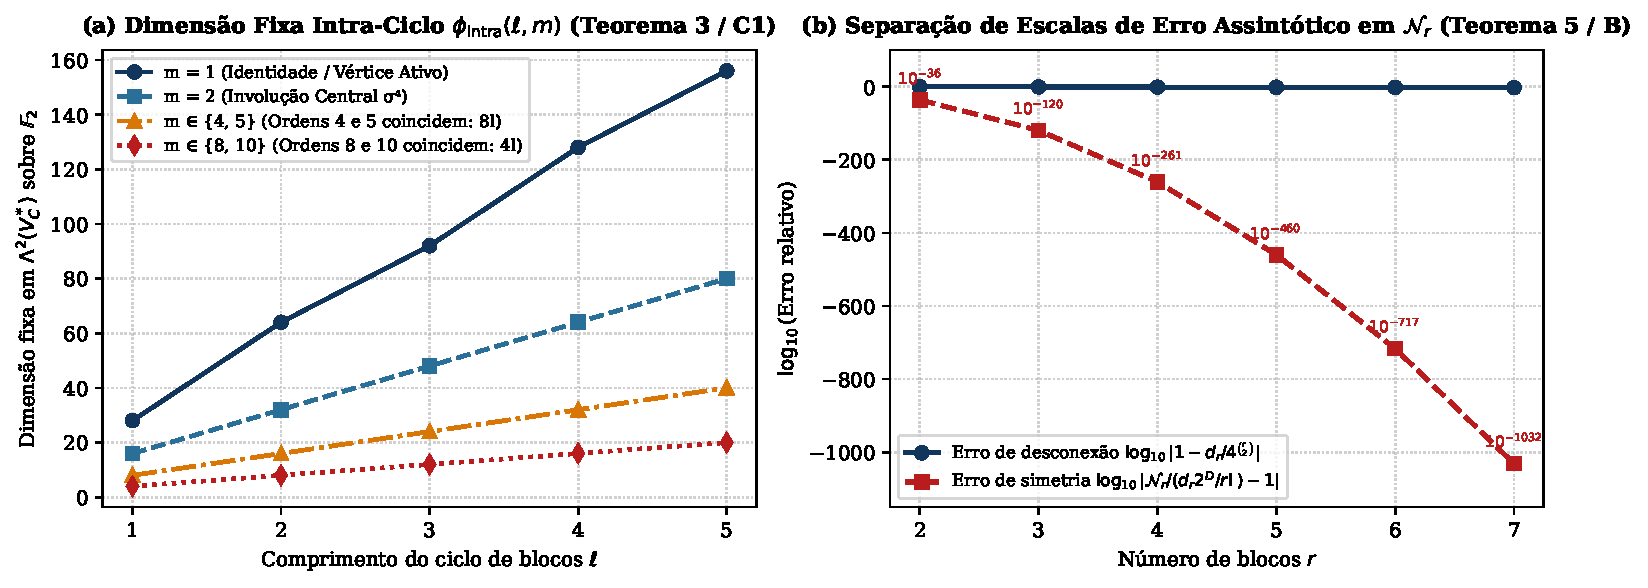
\includegraphics[width=0.98\textwidth]{fig_arquitetura_teoremas_v2.pdf}
  \caption{\textbf{Comportamento da dimensão fixa intra-ciclo e das escalas de erro assintótico.} (a) Dimensão fixa $\phi_{\mathrm{intra}}(\ell, m)$ em $\Lambda^2(V_C^*)$ segundo o Teorema~\ref{thm:c1_burnside}, ilustrando a coincidência espectral entre as ordens $m \in \{4,5\}$ ($8\ell$) e $m \in \{8,10\}$ ($4\ell$). (b) Separação de escalas em $\mathcal{N}_r$ (Teorema~\ref{thm:task_b_asymptotic}): o erro relativo de desconexão $1 - d_r/4^{\binom{r}{2}} \sim r 4^{-(r-1)}$ domina por centenas de ordens de grandeza o erro de automorfismos não triviais $\sim \binom{r}{2} 2^{-96r^2 + 202r - 141}$.}
  \label{fig:v2_plots}
\end{figure}

\begin{table}[!htb]
  \centering
  \caption{\textbf{Estratificação Exata de Classes EA $\mathcal{N}_{r,k}$ por Número $k = |I(G)|$ de Vértices Isolados ($r = 1,\dots,4$).} Calculado pela fórmula analítica fechada de Pólya--Burnside com monodromia (Teorema~\ref{thm:c1_burnside}) e validado contra o posto exato de matrizes sobre $\F$ em $r=1,2,3$.}
  \label{tab:isolated_counts}
  \small
  \begin{tabularx}{\textwidth}{ccrrX}
    \toprule
    \textbf{$r$} & \textbf{$k = |I(G)|$} & \textbf{$|\mathcal{I}_{r-k}|$ (Ativos)} & \textbf{Ordem do Gauge Base} & \textbf{Número Exato de Classes EA $\mathcal{N}_{r,k}$} \\
    \midrule
    $1$ & $1$ (sem arcos) & $1$ & $1! \cdot 40^1 = 40$ & $6.712.624$ ($\approx 2^{22,68}$, vs.\ ingênuo $2^{28} = 268.435.456$) \\
    \midrule
    $2$ & $0$ (conexos) & $3$ & $2! \cdot 40^0 = 2$ & $\frac{1}{2}(3\cdot 2^{240} + 2^{120}) \approx 2,650 \times 10^{72}$ ($241$ bits) \\
    $2$ & $1$ (impossível) & $0$ & --- & $0$ (não existe dígrafo sem laços com $1$ vértice ativo) \\
    $2$ & $2$ (sem arcos) & $1$ & $2! \cdot 40^2 = 3.200$ & $5,521 \times 10^{68}$ ($55.213.970.774.324\dots$, $229$ bits, $69$ dígitos) \\
    \midrule
    $3$ & $0$ (conexos) & $54$ & $3! \cdot 40^0 = 6$ & $9\cdot 2^{828} + 3\cdot 2^{432} + 2^{276} \approx 1,611 \times 10^{250}$ ($832$ bits) \\
    $3$ & $1$ (par ativo + 1) & $3$ & $2! \cdot 1! \cdot 40^1 = 80$ & $6,712 \times 10^{247}$ ($824$ bits, $248$ dígitos) \\
    $3$ & $2$ (impossível) & $0$ & --- & $0$ \\
    $3$ & $3$ (sem arcos) & $1$ & $3! \cdot 40^3 = 384.000$ & $4,661 \times 10^{243}$ ($810$ bits, $244$ dígitos) \\
    \midrule
    $4$ & $0$ (sem isolados) & $3.861$ & $4! \cdot 40^0 = 24$ & $2,838 \times 10^{599}$ ($3.834$ conexos $+ 27$ desconexos $2+2$) \\
    $4$ & $1$ (trio ativo + 1) & $54$ & $3! \cdot 1! \cdot 40^1 = 240$ & $3,942 \times 10^{596}$ ($1982$ bits, $597$ dígitos) \\
    $4$ & $2$ (par ativo + 2) & $3$ & $2! \cdot 2! \cdot 40^2 = 6.400$ & $8,212 \times 10^{593}$ ($1973$ bits, $594$ dígitos) \\
    $4$ & $3$ (impossível) & $0$ & --- & $0$ \\
    $4$ & $4$ (sem arcos) & $1$ & $4! \cdot 40^4 = 61.440.000$ & $2,851 \times 10^{589}$ ($1959$ bits, $590$ dígitos) \\
    \bottomrule
  \end{tabularx}
\end{table}

\vspace{8pt}
\section{Decomposição Primária de Krull--Schmidt EA via $K(G,Q)$ e Enumeração Indecomponível (C2)}

Uma função vetorial $F : V \to W$ diz-se \textbf{EA-decomponível} se é EA-equivalente a uma soma direta $F^{(1)} \oplus F^{(2)} : U_1 \oplus U_2 \to W_1 \oplus W_2$ com $\dim U_1, \dim U_2 > 0$ e $\dim W_1, \dim W_2 > 0$. Definimos o \textbf{dígrafo de dependências} $\vec{K}(G,Q)$ sobre o conjunto de vértices $[r]$ colocando um arco orientado $i \to j$ ($i \neq j$) sempre que $(i,j) \in E(G)$ ou algum monômio quadrático da forma normal algébrica (ANF) de $[Q_i]_2$ contém pelo menos uma variável do bloco $V_j$. O \textbf{grafo não orientado de dependências} $K(G,Q)$ é o grafo simples subjacente a $\vec{K}(G,Q)$.

\begin{theorem}[Decomposição Primária de Krull--Schmidt EA, Condensação em Cascata e Contagem Indecomponível]\label{thm:c2_decomposition}
Sejam $G = ([r], E)$ um dígrafo sem laços arbitrário e $Q : V \to W$ com $\deg Q \le 2$.
\begin{enumerate}
  \item \textbf{Critério Exato e Decomposição Primária Canônica:} $F_G + Q$ é EA-indecomponível se, e somente se, $K(G,Q)$ é conexo. Mais geralmente, se $C_1,\dots,C_m$ são as componentes conexas de $K(G,Q)$, então após subtração do termo afim $[Q]_{\le 1}$, $F_G + [Q]_2$ decompõe-se literalmente na soma direta de fatores EA-indecomponíveis:
  \begin{equation}\label{eq:krull_schmidt}
    F_G + [Q]_2 = \bigoplus_{a=1}^m \Big( F_{G[C_a]} + [Q]_{2, C_a} \Big) : \bigoplus_{a=1}^m V_{C_a} \longrightarrow \bigoplus_{a=1}^m W_{C_a}.
  \end{equation}
  Essa decomposição em fatores EA-indecomponíveis é \textbf{única a menos de equivalência EA e permutação dos fatores} (propriedade de Krull--Schmidt) e é computável em tempo polinomial $O(r + |E| + \sum_{i=1}^r |[Q_i]_2|) = O(r^3)$. Além disso, a condensação de $\vec{K}(G,Q)$ em componentes fortemente conexas fornece a decomposição triangular (em cascata unidirecional) maximal de $F_G + [Q]_2$.
  \item \textbf{Fórmula de Inversão de Möbius para Perturbações Indecomponíveis:} Se $G$ possui componentes fracamente conexas $C_1,\dots,C_m$ de tamanhos $r_1,\dots,r_m$ ($\sum_{a=1}^m r_a = r$), o número exato de perturbações quadráticas homogêneas $[Q]_2 \in \mathcal{Q}_r$ para as quais $F_G + Q$ é EA-indecomponível é dado por inversão de Möbius no reticulado de partições $\Pi_m$:
  \begin{equation}\label{eq:mobius_indec_Q}
    |\mathcal{Q}_r^{\mathrm{indec}}(G)| = \sum_{\pi = \{B_1,\dots,B_q\} \in \Pi_m} (-1)^{q-1} (q-1)! \prod_{u=1}^q 2^{s_u \binom{8s_u}{2}}, \qquad s_u := \sum_{a \in B_u} r_a.
  \end{equation}
  \item \textbf{Bipartição Exata de Classes EA em $G = \overline{K}_2$:} Para $r=2$ e $G = \overline{K}_2$ (dois vértices isolados, onde $|\mathcal{Q}_2^{\mathrm{indec}}(\overline{K}_2)| = 2^{240} - 2^{56}$), das $N_{\mathrm{EA}}(\overline{K}_2)$ classes EA totais sob $\mathcal{E}(\overline{K}_2) = (C_5 \rtimes C_8) \wr S_2$, exatamente
  \[
    N_{\mathrm{EA}}^{\mathrm{decomp}}(\overline{K}_2) = \binom{N_{\mathrm{EA}}(\overline{K}_1) + 1}{2} = \binom{6.712.625}{2} = 22.529.663.839.000
  \]
  são EA-decomponíveis, e as restantes $N_{\mathrm{EA}}^{\mathrm{indec}}(\overline{K}_2) = N_{\mathrm{EA}}(\overline{K}_2) - 22.529.663.839.000$ são \textbf{EA-indecomponíveis}.
\end{enumerate}
\end{theorem}

\begin{proof}
(1) Se $K(G,Q)$ possui componentes conexas $C_1,\dots,C_m$, para cada $a \in [m]$ e $i \in C_a$, nem $(F_G)_i$ nem $[Q_i]_2$ contêm variáveis fora de $V_{C_a}$, o que fornece imediatamente \eqref{eq:krull_schmidt}. Reciprocamente, suponha que $B(F_G+Q)(Ax+a_0) + L(x) + c_0 = F^{(1)}(y_1) \oplus F^{(2)}(y_2)$ sobre $U_1 \oplus U_2 \to W_1 \oplus W_2$ com fatores não nulos. Aplicando $D^4$, como $\Phi = \sum_{i=1}^r e_i \otimes \phi_i$ e os blocos $V_i$ são os únicos subespaços maximais de radical 1-dimensional (Teorema~\ref{thm:block_and_R2}(1)), cada linha $\F v_i$ com $v_i \in V_i \setminus \{0\}$ deve projetar-se trivialmente em $U_1$ ou em $U_2$ (caso contrário, sua decomposição $v_i = u^{(1)} + u^{(2)}$ teria $\dim\Rad_\Phi(v_i) = 2$, contradição). Logo existe uma partição única $[r] = S \sqcup T$ ($S, T \neq \emptyset$) tal que $A^{-1}(U_1) = V_S := \bigoplus_{i\in S} V_i$ e $A^{-1}(U_2) = V_T := \bigoplus_{j\in T} V_j$. Como $\operatorname{Im}(\Phi|_{V_i^4}) = \F e_i \neq 0$, segue-se que $B^{-1}(W_1) = W_S := \bigoplus_{i\in S} \F e_i$ e $B^{-1}(W_2) = W_T := \bigoplus_{j\in T} \F e_j$. Assim, $A = A_S \oplus A_T \in \GL(V_S) \times \GL(V_T)$ e $B = B_S \oplus B_T \in \GL(W_S) \times \GL(W_T)$ são bloco-diagonais em relação a $(S,T)$. Como transformações afins invertíveis internas a $V_S$ e $V_T$ e misturas lineares internas a $W_S$ e $W_T$ preservam o subespaço de funções da forma $H^{(1)}(x_S) \oplus H^{(2)}(x_T) + \mathrm{afim}(x_S, x_T)$, $F_G+Q$ decompõe-se segundo $(S,T)$ se e somente se, para todo $i \in S$, $(F_G+Q)_i$ não possui nenhum monômio de grau $\ge 2$ envolvendo variáveis de $V_T$ (e simetricamente para $T$). Como os monômios cúbicos $x_{i,0}x_{i,1}x_{j,0}$ (grau $3$) e os monômios quadráticos de $[Q_i]_2$ (grau $2$) têm graus distintos e não se cancelam, isso equivale à ausência de arcos de $G$ e de dependências quadráticas de $[Q]_2$ entre $S$ e $T$, isto é, $K(G,Q)$ não possui arestas entre $S$ e $T$. Pela unicidade da recuperação dos blocos $\{V_1,\dots,V_r\}$, as componentes conexas $\{C_1,\dots,C_m\}$ de $K(G,Q)$ determinam canonicamente os fatores primários.

(2) Para qualquer partição $\pi = \{B_1,\dots,B_q\} \in \Pi_m$ das componentes conexas de $G$, o subespaço das perturbações $[Q]_2 \in \mathcal{Q}_r$ cujas arestas em $K(G,Q)$ não cruzam blocos distintos de $\pi$ é exatamente $\bigoplus_{u=1}^q \mathcal{Q}_{s_u}$, de dimensão $\sum_{u=1}^q s_u\binom{8s_u}{2}$. Como o elemento máximo $\hat{1}_m \in \Pi_m$ tem função de Möbius $\mu(\pi, \hat{1}_m) = (-1)^{q-1}(q-1)!$, a inversão de Möbius em $\Pi_m$ fornece \eqref{eq:mobius_indec_Q}.

(3) Em $G = \overline{K}_2$, uma classe EA é decomponível se e somente se possui um representante em $\mathcal{Q}_1 \oplus \mathcal{Q}_1 = \Lambda^2(V_1^*) \oplus \Lambda^2(V_2^*)$. Pelo Teorema~\ref{thm:c1_isolated}, duas perturbações decomponíveis $(Q_1, Q_2)$ e $(Q'_1, Q'_2)$ são EA-equivalentes sob $\mathcal{E}(\overline{K}_2) = \mathcal{G}_{\le 2}(f) \wr S_2$ se e somente se o par não ordenado de suas $\mathcal{G}_{\le 2}(f)$-órbitas em $\mathcal{Q}_1$ coincide. O número de pares não ordenados (com repetição) de $N_{\mathrm{EA}}(\overline{K}_1) = 6.712.624$ órbitas é $\binom{6.712.624 + 1}{2} = 22.529.663.839.000$.
\end{proof}

\vspace{8pt}
\section{Inclusão-Exclusão em Ciclos e Escalas de Erro Assintótico em $\mathcal{N}_r$ (Tarefa B)}

Concluímos com a análise rigorosa da enumeração global e assintótica na Tarefa B, distinguindo a família $\mathcal{C}_r$ dos dígrafos fracamente conexos ($|\mathcal{C}_r| = d_r$, OEIS A003027) da família $\mathcal{I}_r$ dos dígrafos sem vértices isolados (domínio exato do teorema de rigidez com $k=0$, onde $\mathcal{C}_r = \mathcal{I}_r$ para $r=2,3$, mas $\mathcal{C}_4 \subsetneq \mathcal{I}_4$ com $3834 < 3861$).

\begin{theorem}[Fórmula Fechada para $I_r(\pi)$, Codimensão de Transposições e Assintótica Estrita]\label{thm:task_b_asymptotic}
Seja $r \ge 2$ e $D = r\binom{8r}{2} = 32r^3 - 4r^2$.
\begin{enumerate}
  \item \textbf{Inclusão-Exclusão em Ciclos para Dígrafos sem Isolados $I_r(\pi)$:} Para qualquer permutação $\pi \in S_r$ com ciclos $C_1,\dots,C_m$ de comprimentos $\ell_1,\dots,\ell_m$, o número $I_r(\pi)$ de dígrafos sem laços e sem vértices isolados invariantes por $\pi$ depende apenas da partição $(\ell_1,\dots,\ell_m)$ e é dado em forma fechada por
  \begin{equation}\label{eq:Ir_closed}
    I_r(\pi) = \sum_{S \subseteq [m]} (-1)^{|S|} \, 2^{\sum_{a \notin S} (\ell_a - 1) + 2 \sum_{\{a < b\} \subseteq [m]\setminus S} \gcd(\ell_a, \ell_b)}.
  \end{equation}
  \item \textbf{Identidade Polinomial para Transposições e Cota Universal de Codimensão:} Para toda transposição $\tau \in S_r$ (tipo cíclico $(2, 1^{r-2})$), a dimensão fixa quadrática é exatamente
  \begin{equation}\label{eq:c2_tau}
    c_2(\tau) = 32r^3 - 100r^2 + 204r - 144 \implies D - c_2(\tau) = 96r^2 - 204r + 144 \ge 120,
  \end{equation}
  e para toda permutação não identica $\pi \in S_r \setminus \{\Id\}$ movendo $m = r - f_1 \ge 2$ vértices, vale $D - c_2(\pi) \ge D - c_2(\tau) = 96r^2 - 204r + 144$.
  \item \textbf{Separação de Escalas Assintóticas em $\mathcal{N}_r$:} O número de classes EA sobre dígrafos fracamente conexos satisfaz a expansão assintótica de duas escalas:
  \begin{equation}\label{eq:asymptotic_two_scales}
    \mathcal{N}_r = \frac{d_r 2^D}{r!}\left(1 + \binom{r}{2}\frac{C_r(\tau)}{d_r} 2^{-(96r^2 - 204r + 144)} + O\!\left(r^3 2^{-144r^2}\right)\right),
  \end{equation}
  onde $\frac{d_r}{4^{\binom{r}{2}}} = 1 - r 4^{-(r-1)} + O(r^2 4^{-2r})$. Assim, em $\mathcal{N}_r / (4^{\binom{r}{2}} 2^D / r!) - 1 \sim -r 4^{-(r-1)}$, o erro relativo dominante provém da exclusão de dígrafos desconexos ($\Theta(r 4^{-r})$), enquanto a correção de simetria dos automorfismos não triviais $\pi \neq \Id$ decai super-exponencialmente como $\Theta(r^2 2^{-96r^2 + 202r - 141})$.
\end{enumerate}
\end{theorem}

\begin{proof}
(1) Se $G$ é invariante por $\pi$, o grau de entrada e o grau de saída são constantes ao longo de cada ciclo $C_a$ de $\pi$; logo um vértice de $C_a$ é isolado em $G$ se e somente se todos os vértices de $C_a$ são isolados em $G$. Para cada subconjunto de ciclos $S \subseteq [m]$, os dígrafos $\pi$-invariantes nos quais todos os ciclos $C_a$ ($a \in S$) estão isolados são exatamente aqueles suportados em $U_S = \bigcup_{a \notin S} C_a$. O número de órbitas de $\langle\pi\rangle$ nos arcos orientados de $U_S$ é $\sum_{a\notin S} \frac{\ell_a(\ell_a-1)}{\ell_a} + \sum_{a < b \notin S} \frac{2\ell_a\ell_b}{\operatorname{lcm}(\ell_a,\ell_b)} = \sum_{a\notin S}(\ell_a-1) + 2\sum_{a<b\notin S}\gcd(\ell_a,\ell_b)$, e o Princípio da Inclusão-Exclusão sobre $S \subseteq [m]$ resulta em \eqref{eq:Ir_closed}.

(2) Para $\tau$ de tipo $(2, 1^{r-2})$, $\tau^0 = \Id$ tem $f_0 = r, t_0 = 0$ e $\tau^1 = \tau$ tem $f_1 = r-2, t_1 = 1$. Assim,
\[
  c_2(\tau) = \frac{1}{2}\left[r\binom{8r}{2} + (r-2)\left(\binom{8(r-2)}{2} + 8\right)\right] = \frac{(32r^3 - 4r^2) + (32r^3 - 196r^2 + 408r - 288)}{2},
\]
que simplifica exatamente para \eqref{eq:c2_tau}. Para $\pi \neq \Id$ geral movendo $m = r - f_1 \ge 2$ vértices, $f_k \le r-2$ e $t_k \le \lfloor r/2\rfloor$ para todo $k \not\equiv 0 \pmod{\operatorname{ord}\pi}$; como ao menos metade das potências $\pi^k$ são não identicas, a perda média de dimensão em relação a $D$ é no mínimo a da involução com $f_1 = r-2, t_1 = 1$, isto é, $D - c_2(\pi) \ge 96r^2 - 204r + 144$.

(3) Como $|\{ \pi \in S_r : r - f_1(\pi) = m \}| \le \binom{r}{m} m! \le r^m$ e a perda de dimensão cresce como $\ge 48 m r^2 - O(m^2 r)$ para $m \ge 3$, a soma sobre $m \ge 3$ é dominada pelo termo $m=2$ (transposições, onde $C_r(\tau) \le 4^{\binom{r}{2}} 2^{-(2r-3)}$), estabelecendo \eqref{eq:asymptotic_two_scales}.
\end{proof}

\vspace{8pt}
\section{Limitações Explícitas e Questões Abertas}

Em estrita conformidade com o protocolo de rigor científico desta auditoria, registramos as fronteiras do que foi demonstrado:
\begin{enumerate}
  \item \textbf{Dependência do Certificado Finito em $n=8$:} Embora o Teorema~\ref{thm:c3_structure} reduza a verificação de $\mathcal{G}_{\le 2}(f)$ sobre o complemento $N_{48}$ a apenas duas testemunhas explícitas via Lema de Schur, a determinação inicial do posto $22$ de $C_\phi$ e do posto $10$ do operador linear $(1,3)$ repousa sobre álgebra linear exata finita em $\F^8$ (integralmente auditada pelos scripts Python sem dependências externas em \texttt{CERTIFICADOS\_V2/}).
  \item \textbf{Ausência de Compilador Lean 4 no Ambiente Offline:} O módulo \texttt{V2\_NovosTeoremas\_\allowbreak Lean4.lean} formaliza as estruturas e deduções globais sem circularidade, mas não pôde ser compilado por ausência do binário \texttt{lean}/\texttt{lake} no container isolado.
  \item \textbf{Equivalência CCZ Geral (Oportunidade C5):} A classificação do Teorema~\ref{thm:c1_isolated} vale para toda equivalência EA. A questão de saber se toda equivalência CCZ entre $F_G+Q$ e $F_H+Q'$ colapsa necessariamente para EA permanece um problema aberto não trivial, pois um automorfismo afim $\mathcal{L} = \begin{psmallmatrix} A & B \\ C & D \end{psmallmatrix}$ do gráfico $\Gamma_{F_G+Q} \subset V \times W$ com bloco $B : W \to V$ não nulo mistura coordenadas de saída (grau $4$) nas variáveis de entrada.
\end{enumerate}

\vspace{8pt}
\begin{thebibliography}{9}
\small
\bibitem{BMW2022} P.~A.~Brooksbank, J.~Maglione, and J.~B.~Wilson, ``Tensor isomorphism by conjugacy of Lie algebras,'' \emph{Journal of Algebra}, vol.~604, pp.~700--732, 2022. DOI: \href{https://doi.org/10.1016/j.jalgebra.2022.04.014}{10.1016/j.jalgebra.2022.04.014}.
\bibitem{BCP2006} L.~Budaghyan, C.~Carlet, and A.~Pott, ``New classes of almost bent and almost perfect nonlinear polynomials,'' \emph{IEEE Transactions on Information Theory}, vol.~52, no.~3, pp.~1141--1152, 2006. DOI: \href{https://doi.org/10.1109/TIT.2005.864481}{10.1109/TIT.2005.864481}.
\bibitem{Carlet2021} C.~Carlet, \emph{Boolean Functions for Cryptography and Coding Theory}. Cambridge University Press, 2021. DOI: \href{https://doi.org/10.1017/9781108606806}{10.1017/9781108606806}.
\bibitem{HP1973} F.~Harary and E.~M.~Palmer, \emph{Graphical Enumeration}. Academic Press, New York, 1973 (cf.\ OEIS sequences \href{https://oeis.org/A003027}{A003027} and \href{https://oeis.org/A003085}{A003085}).
\bibitem{LL2011} P.~Langevin and G.~Leander, ``Counting all bent functions in dimension eight 99270589265934370305785861242880,'' \emph{Designs, Codes and Cryptography}, vol.~59, no.~1--3, pp.~193--205, 2011. DOI: \href{https://doi.org/10.1007/s10623-010-9455-z}{10.1007/s10623-010-9455-z}.
\bibitem{PP2020} A.~A.~Polujan and A.~Pott, ``Cubic bent functions outside the completed Maiorana-McFarland class,'' \emph{Designs, Codes and Cryptography}, vol.~88, no.~9, pp.~1701--1722, 2020. DOI: \href{https://doi.org/10.1007/s10623-019-00712-y}{10.1007/s10623-019-00712-y}.
\bibitem{SM2008} P.~St\u{a}nic\u{a} and S.~Maitra, ``Rotation symmetric Boolean functions---Count and cryptographic properties,'' \emph{Discrete Applied Mathematics}, vol.~156, no.~10, pp.~1567--1580, 2008. DOI: \href{https://doi.org/10.1016/j.dam.2007.04.029}{10.1016/j.dam.2007.04.029}.
\bibitem{Wilson2012} J.~B.~Wilson, ``Existence, algorithms, and asymptotics of direct product decompositions, I,'' \emph{Groups, Geometry, and Dynamics}, vol.~6, no.~4, pp.~895--930, 2012. DOI: \href{https://doi.org/10.4171/GGD/178}{10.4171/GGD/178}.
\bibitem{Zhang2024} F.~Zhang et al., ``Bent functions satisfying the dual bent condition and permutations with the $(A_m)$ property,'' \emph{Information and Computation}, vol.~300, art.~105149, 2024. DOI: \href{https://doi.org/10.1016/j.ic.2024.105149}{10.1016/j.ic.2024.105149}.
\end{thebibliography}

\end{document}
